\ifSTANDALONE
\section{Firmware}
\fi
\ifEMBED
\subsubsection{Firmware}
\label{sec:ET_Firmware}
\fi
\ifSTANDALONE
\subsection{Übersicht}
\fi
\ifEMBED
\paragraph{Übersicht}$~~$\vspace{2mm}\\
\fi
Die Firmware des Boards erfüllt mehrere Aufgaben. Während dem Anfahren des Motors realisiert
sie die Zwangskommutierung, im Nennbetrieb regelt sie die Drehzahl des
Motors. Sobald der Motor in Betrieb ist, wir die Kommutierung mittes Interrupts hardwaremässig
realisiert.
\ifSTANDALONE
\subsection{Takt}
\fi
\ifEMBED
\paragraph{Takt}$~~$\vspace{2mm}\\
\fi
Der Referenztakt wird durch einen Quarz mit einer Frequenz von 
12\si{\mega\hertz} erzeugt.  Dieser Takt dient als Referenztakt für die PLL\footnote{phase-locked loop, eine elektronische Schaltung, die die Phasenlage und Frequenz beeinflussen kann} 
des HS9S08JM60. Dazu wird er durch acht geteilt um im erlaubten 
Bereich\footnote{Die Frequenz des Eingangssignals der PLL muss im Bereich 1 
\ldots 2\si{\mega\hertz} liegen. \cite[p.  195]{Datasheet:HCS08}} für die PLL 
zu liegen. In der PLL wird der Takt mit 32 multipliziert. Dies ergibt einen 
CPU Takt von 48\si{\mega\hertz}. Da der Bustakt der Hälfte des CPUtakts 
entspricht, weist dieser eine Frequenz von 24\si{\mega\hertz} auf.  Der 
Externe Takt (16\si{\mega\hertz}) wird zusätzlich als externer Referenztakt 
zur Verfügung gestellt und vom RTC verwendet.  (siehe auch Abschnitt 
\ref{sec:rtc} \nameref{sec:rtc})

\ifSTANDALONE
\subsection{RTC}
\fi
\ifEMBED
\paragraph{RTC}$~~$\vspace{2mm}\\
\fi
\label{sec:rtc}
Um regelmässig abzuarbeitende Aufgaben zu steuern, wird ein entsprechender 
Takt benötigt. Dafür wird der RTC\footnote{\textbf{R}eal \textbf{T}ime 
\textbf{Counter}} verwendet. Dieser verwendet als Takt den externen 
Referenztakt mit einer Frequenz von 16\si{\mega\hertz}. Dieser wird mit dem 
Prescaler auf eine Frequenz von 16\si{\kilo\hertz} geteilt. Über das Modulo 
Register kann eine Periodendauer im Bereich 62.5\si{\micro\second} \ldots 
16\si{\milli\second} eingestellt werden. Es wird zunächst eine Periodendauer 
von 1\si{\milli\second} verwendet. In der ISR\footnote{\textbf{I}nterrupt 
\textbf{S}ervice \textbf{Routine}} wird ein Flag gesetzt, welches in der 
Hauptschlaufe abgefragt wird. 
%\begin{table}[h!]
%    \begin{zebratabular}{p{0.10\textwidth}p{0.06\textwidth}p{0.25\textwidth}p{0.5\textwidth}}
%    \rowcolor{gray} Register & Wert & Beschreibung & Bemerkungen \\
%    RTCSC &
%        \verb!0x38! &
%        RTC Status and Control Register &
%        ERCLK, Interrupts enabled, Prescaler = $10^3$ $\to$ T$_{\text{Count}}$ = $\frac{1}{16}$\si{\milli\second} \\
%    RTCMOD &
%        \verb!0x0F! &
%        RTC Modulo Register &
%        Modulo = 15 $\to$ T$_{\text{Interrupt}}$ = 1\si{\milli\second} \\
%    \end{zebratabular}
%    \caption{Registerinitialisierung RTC}
%    \label{tab:rtc_init}
%\end{table}

\ifSTANDALONE
\subsection{PWM}
\fi
\ifEMBED
\paragraph{PWM}$~~$\vspace{2mm}\\
\fi
Mit der PWM werden 
die Ausgangsstufen angesteuert. Über das Puls - Pausenverhältnis wird die 
Leistung eingestellt. Damit diese Ansteuerung jedoch nicht hörbar wird, muss 
der Motor mit einer PWM Frequenz oberhalb des hörbaren Frequenzbereichs des 
Menschen angesteuert werden. Es wird eine Frequenz von 24\si{\kilo\hertz} 
verwendet.  Für das Erzeugen der PWM wird der Timer TPM2 verwendet. 
%\begin{table}[h!]
%    \begin{zebratabular}{p{0.10\textwidth}p{0.06\textwidth}p{0.25\textwidth}p{0.5\textwidth}}
%    \rowcolor{gray} Register & Wert & Beschreibung & Bemerkungen \\
%    TPM2SC &
%        \verb!0x08! &
%        TPM2 Status and Control Register &
%        Overflow interrupt disabled, no Center-aligned PWM, Bus clock as clock 
%            source, Prescaler = 1\\
%    TPM2CNT &
%        \verb!0x____! &
%        TPM2 Counter Register &
%        No initialisation \\
%    TPM2MOD &
%        \verb!0x03FF! &
%        TPM2 Counter Modulo Register &
%        1023 $\to$ $\frac{24\si{\mega\hertz}}{1024} = 23.4375\si{\kilo\hertz}$  \\
%    TPM2C0SC &
%        \verb!0x28! &
%        TPM2 Channel 0 Status and Control Register &
%        Interrupt disabled, edge aligned PWM, High-true\\
%    TPM2C0V &
%        \verb!0x0033! &
%        TPM2 Channel 0 Value Register &
%        5\si{\percent} \\
%    TPM2C1SC &
%        \verb!0x24! &
%        TPM2 Channel 1 Status and Control Register &
%        Interrupt disabled, edge aligned PWM, Low-true\\
%    TPM2C1V &
%        \verb!0x03CD! &
%        TPM2 Channel 1 Value Register &
%        5\si{\percent} \\
%    \end{zebratabular}
%    \caption{Registerinitialisierung TPM2}
%    \label{tab:rtc_init}
%\end{table}

\ifSTANDALONE
\subsection{Kommutierungsverzögerung / Zeitmessung}
\fi
\ifEMBED
\paragraph{Kommutierungsverzögerung / Zeitmessung}$~~$\vspace{2mm}\\
\fi
Um den exakten Kommutierungszeitpunkt einstellen zu können und um die Zeit 
zwischen zwei Kommutierungen zu messen, wird ein weiterer Timer benötigt. Dafür 
wird TPM1 benutzt. Als Taktquelle für den Timer wird der Bustakt mit einer 
Frequenz von 24\si{\mega\hertz} verwendet. Dieser wird mit dem maximal möglichen 
Prescaler von 128 geteilt. Dies ergibt eine Frequenz von 187.5\si{\kilo\hertz} 
und eine Auflösung von 5.33\si{\micro\second}. Damit ist eine maximale 
Messdauer von 349.5\si{\milli\second} möglich. 
%\begin{table}[h!]
%    \begin{zebratabular}{p{0.10\textwidth}p{0.06\textwidth}p{0.25\textwidth}p{0.5\textwidth}}
%    \rowcolor{gray} Register & Wert & Beschreibung & Bemerkungen \\
%    TPM1SC &
%        \verb!0x0F! &
%        TPM1 Status and Control Register &
%        Overflow interrupt disabled, no Center-aligned PWM, Bus clock as clock 
%            source, Prescaler = 128\\
%    TPM1CNT &
%        \verb!0x____! &
%        TPM1 Counter Register &
%        No initialisation \\
%    TPM1MOD &
%        \verb!0x0000! &
%        TPM1 Counter Modulo Register &
%        Free running \\
%    TPM1C0SC &
%        \verb!0x50! &
%        TPM1 Channel 0 Status and Control Register &
%        Interrupt enabled, Output compare \\
%    TPM1C0V &
%        \verb!0x0000! &
%        TPM1 Channel 0 Value Register &
%        Used for commutation delay of phase U \\
%    TPM1C1SC &
%        \verb!0x50! &
%        TPM1 Channel 1 Status and Control Register &
%        Interrupt enabled, Output compare \\
%    TPM1C1V &
%        \verb!0x0000! &
%        TPM1 Channel 1 Value Register &
%        Used for commutation delay of phase V \\
%    TPM1C2SC &
%        \verb!0x50! &
%        TPM1 Channel 2 Status and Control Register &
%        Interrupt enabled, Output compare \\
%    TPM1C2V &
%        \verb!0x0000! &
%        TPM1 Channel 2 Value Register &
%        Used for commutation delay of phase W \\
%    TPM1C3SC &
%        \verb!0x44! &
%        TPM1 Channel 3 Status and Control Register &
%        Interrupt enable, input capture \\
%    TPM1C3V &
%        \verb!0x0000! &
%        TPM1 Channel 3 Value Register &
%        Initialized zero, value not used later \\
%    TPM1C4SC &
%        \verb!0x44! &
%        TPM1 Channel 4 Status and Control Register &
%        Interrupt enable, input capture \\
%    TPM1C4V &
%        \verb!0x0000! &
%        TPM1 Channel 4 Value Register &
%        Initialized zero, value not used later \\
%    TPM1C5SC &
%        \verb!0x44! &
%        TPM1 Channel 5 Status and Control Register &
%        Interrupt enable, input capture \\
%    TPM1C5V &
%        \verb!0x0000! &
%        TPM1 Channel 5 Value Register &
%        Initialized zero, value not used later \\
%    \end{zebratabular}
%    \caption{Registerinitialisierung TPM1}
%    \label{tab:rtc_init}
%\end{table}

\ifSTANDALONE
\subsection{Kommunikation zum Host}
\fi
\ifEMBED
\paragraph{Kommunikation zum Host}$~~$\vspace{2mm}\\
\fi
Zur Interaktion mit dem BLDC-Board wird die SPI1-Schnittstelle des $\mu C$ verwendet. Dabei
ist das SPI-Interface im 8 Bit Mode mit LSB-First konfiguriert. Zusätzlich zu dieser Schnittstelle
ist eine IRQ-Leitung vorhanden, mit der das BLDC-Board den Host triggern kann, um auf ein Problem 
hinzuweisen. Die Steckerbelegung ist in Tabelle \ref{tab:SPI_stecker} ersichtlich.
%\begin{table}[h!]
%    \begin{zebratabular}{p{0.10\textwidth}p{0.06\textwidth}p{0.25\textwidth}p{0.5\textwidth}}
%    \rowcolor{gray} Register & Wert & Beschreibung & Bemerkungen \\
%    SPI1C2 &
%        \verb!0x00! &
%        SPI Control Register 2 & 
%        \\
%    SPI1C1 &
%        \verb!0x85! &
%        SPI Control Register 1 &
%        IRQ-Enable aktiviert und LSB-First konfiguriert\\
%    \end{zebratabular}
%    \caption{Registerinitialisierung SPI1}
%    \label{tab:spi1_init}  
%\end{table}

\begin{table}[h!]
    \begin{zebratabular}{p{0.10\textwidth}p{0.06\textwidth}}
    \rowcolor{gray} Pin & Name\\
    1 & GND\\
    2 & MISO\\
    3 & CS\\
    4 & MOSI\\
    5 & CLK\\
    6 & IRQ\\
    \end{zebratabular}
    \centering
    \caption{Steckerbelegung der SPI-Schnittstelle}
    \label{tab:SPI_stecker}
\end{table}
Die Kommunikation zwischen BLDC-Board und Host funktioniert über ein Protokoll zur Interaktion. Die 
Spezifikation dieses Protokolls ist in der Tabelle \ref{tab:Spi_Int_Table} ersichtlich. Das obere Nibble des
CMD's\footnote{Command-Byte, ein spezielles Byte, das zur Signalisation von Befehlen verwendet wird} 
enthält den Befehl und das untere Nibble die Anzahl Argumente, die zum CMD gehören.
Wenn das untere Nibble \verb!0xF! ist, wird die Länge der Übertragung im nächsten Byte signalisiert.

\ifSTANDALONE
    \begin{table}[h!]
    \begin{zebratabular}{p{0.12\textwidth}p{0.06\textwidth}p{0.35\textwidth}p{0.4\textwidth}}
\fi
    \ifEMBED
    \begin{zebralongtable}{p{0.12\textwidth}p{0.06\textwidth}p{0.35\textwidth}p{0.4\textwidth}}
        \caption{Kommunikationsprotokoll}
        \endlastfoot
\fi
    \rowcolor{gray} Name & Wert & Beschreibung & Parameter\\
    Dummy &
        \verb!0x00! & 
        Byte das benötigt wird, um zu clocken für die Übertragung von Argumenten &
        \\
    Start &
        \verb!0x10! & 
        Startet den Motor &
        \\
    Stop &
        \verb!0x20! & 
        Stoppt den Motor &
        \\
    setRPM &
        \verb!0x32! & 
        16 Bit Zahl um die Drehzahl einzustellen & 
        1. Byte = High-Byte\newline 
        2. Byte = Low-Byte\\
    setVoltage &
        \verb!0x42! & 
        $U_{GS}$ der FET's. & 1. Byte = Spannungswert-High-Byte\newline 
                              2. Byte = Spannungswert-Low-Byte\\
    setCurrent &
        \verb!0x51! & 
        Wert der Strombegrenzung. Der Stromwert ergibt sich nach der Formel $Current = Wert \cdot 10$ &
        $Registerwert = \frac{Sollwert\; in \;[mA]}{10} $\\
    getStatus &
        \verb!0x64! & 
        Gibt der Board-Status zurück &
        1. Byte = Motor-Status\newline
        2. Byte = Fehler-Code\newline
        3. Byte = RPM-High-Byte\newline
        4. Byte = RPM-Low-Byte\\
    areYouAlive &
        \verb!0x71! & 
        Damit kann die Kommunikation und das BLDC-Board testen &
        Das BLDC-Board gibt \verb!0x55! zurück\\
    setPwm &
        \verb!0x81! & 
        Damit kann die PWM des Motors eingestllt werden &
        PWM-Wert im Bereich 1-100 \% \\
    startMessung Param &
        \verb!0xC3! & 
        Messung parametrisiert starten &
        1. Byte = Pulsdauer\newline
        2. Byte = RPM-High-Byte\newline
        3. Byte = RPM-Low-Byte\\
    startMessung &
        \verb!0xD0! & 
        Messung mit einem Schritt starten &
        \\
    getMessung &
        \verb!0xEF! & 
        gibt die gespeicherte Messung zurück &
        1. Byte = Länge\newline
        2. - n. Byte = Daten der Messung
\ifSTANDALONE
    \end{zebratabular}
    \caption{Kommunikationsprotokoll}
    \label{tab:Spi_Int_Table}
    \end{table}
\fi
\ifEMBED
    \label{tab:Spi_Int_Table}
    \end{zebralongtable}
\fi

\ifSTANDALONE
\subsection{Regler}
\fi
\ifEMBED
\paragraph{Regler}$~~$\vspace{2mm}\\
\fi
In der Software ist ein PID-Regler mit Vorsteuerung implementiert. Dies ist im Blockschema in der 
Abbildung \ref{abb:BlockschemaRegler} abgebildet. Je nachdem Wahl der Parameter $P$, $I$, $D$ und 
$F_{Forward}$, können nur einzelne Teile des Reglers verwendet werden. 
\ifSTANDALONE
Auf diese weise kann zum Beispiel ein PI-Regler realisiert werden. 
\fi 
\ifEMBED
Während der Testphase, siehe Testbericht in Kapitel \ref{sec:ParameterSuche}, stellte sich heraus, 
dass ein reiner PI-Regler ohne Feedforward den Anforderungen am besten entsprechen. somit sind die 
Parameter $D = 0$ und $F_{Forward} = 0$.
\fi
Als Feedback wird die Zeit, die für die 
Kommutierung bereist besprochen wurde, verwendet. Damit kurzfristige Unregelmässigkeiten gedämpft 
werden, wird das Feedback durch ein FIR-Filter\footnote{Finite Impulse Response Filter, Ein Filter 
mit garantierter endlichen Antwort auf ein Impuls} gefiltert. Der Ausgang dieses Filters wird mittels 
eines Korrekturfaktor in RPM umgerechnet. Dieser Wert wird mit der Stellgrösse verrechnet und dem Regler 
zugeführt.
\begin{figure}[h!]
    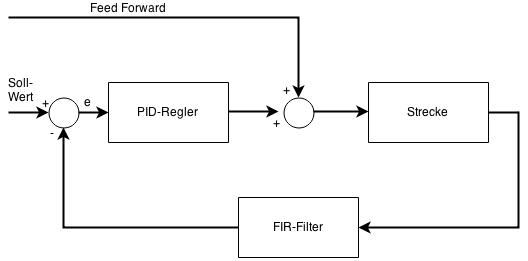
\includegraphics[width=0.6\textwidth,clip,trim=0mm 0mm 0mm 0mm]
    {\EtPath/Bilder/Blockschaltbild_Regler.jpg}
    \centering
    \caption{Blockschema der Regelung}
    \label{abb:BlockschemaRegler}
\end{figure}

%\begin{table}[h!]
%    \begin{zebratabular}{p{0.07\textwidth}p{0.07\textwidth}p{0.07\textwidth}p{0.07\textwidth}p{0.07\textwidth}p{0.07\textwidth}p{0.07\textwidth}p{0.07\textwidth}}
%    \rowcolor{gray} \multicolumn{8}{|c|}{Mögliche Werte als Argument für setVoltage }\\
%    $60 mV$   & $68 mV$   & $76 mV$   & $86 mV$   & $97 mV$   & $109 mV$  & $123 mV$  & $138 mV$  \\
%    $155 mV$  & $175 mV$  & $197 mV$  & $222 mV$  & $250 mV$  & $282 mV$  & $317 mV$  & $358 mV$  \\
%    $403 mV$  & $454 mV$  & $511 mV$  & $576 mV$  & $648 mV$  & $730 mV$  & $822 mV$  & $926 mV$  \\
%    $1046 mV$ & $1175 mV$ & $1324 mV$ & $1491 mV$ & $1679 mV$ & $1892 mV$ & $2131 mV$ & $2400 mV$ \\
%    \end{zebratabular}
%        \centering
%    \caption{Gültige Wert als Argument für setVoltage}
%\end{table}

